\section{Implementation}

\begin{figure}[H]
    \centering
    \caption{Module Diagram}
\end{figure}

\subsection{8-bit DAC Hardware}

A relatively high quality DAC is required in order to synthesize composite
video. AD9748 was selected as it had a fast rise and fall time, parallel input,
and up to 210 MSPS. The only challenge was that no breakout boards existed for
this IC, so a general breakout board was ordered for the QFN-32 package, and
with some help from Ed Casas we managed to reflow solder the IC successfully:

\begin{figure}[H]
    \centering
    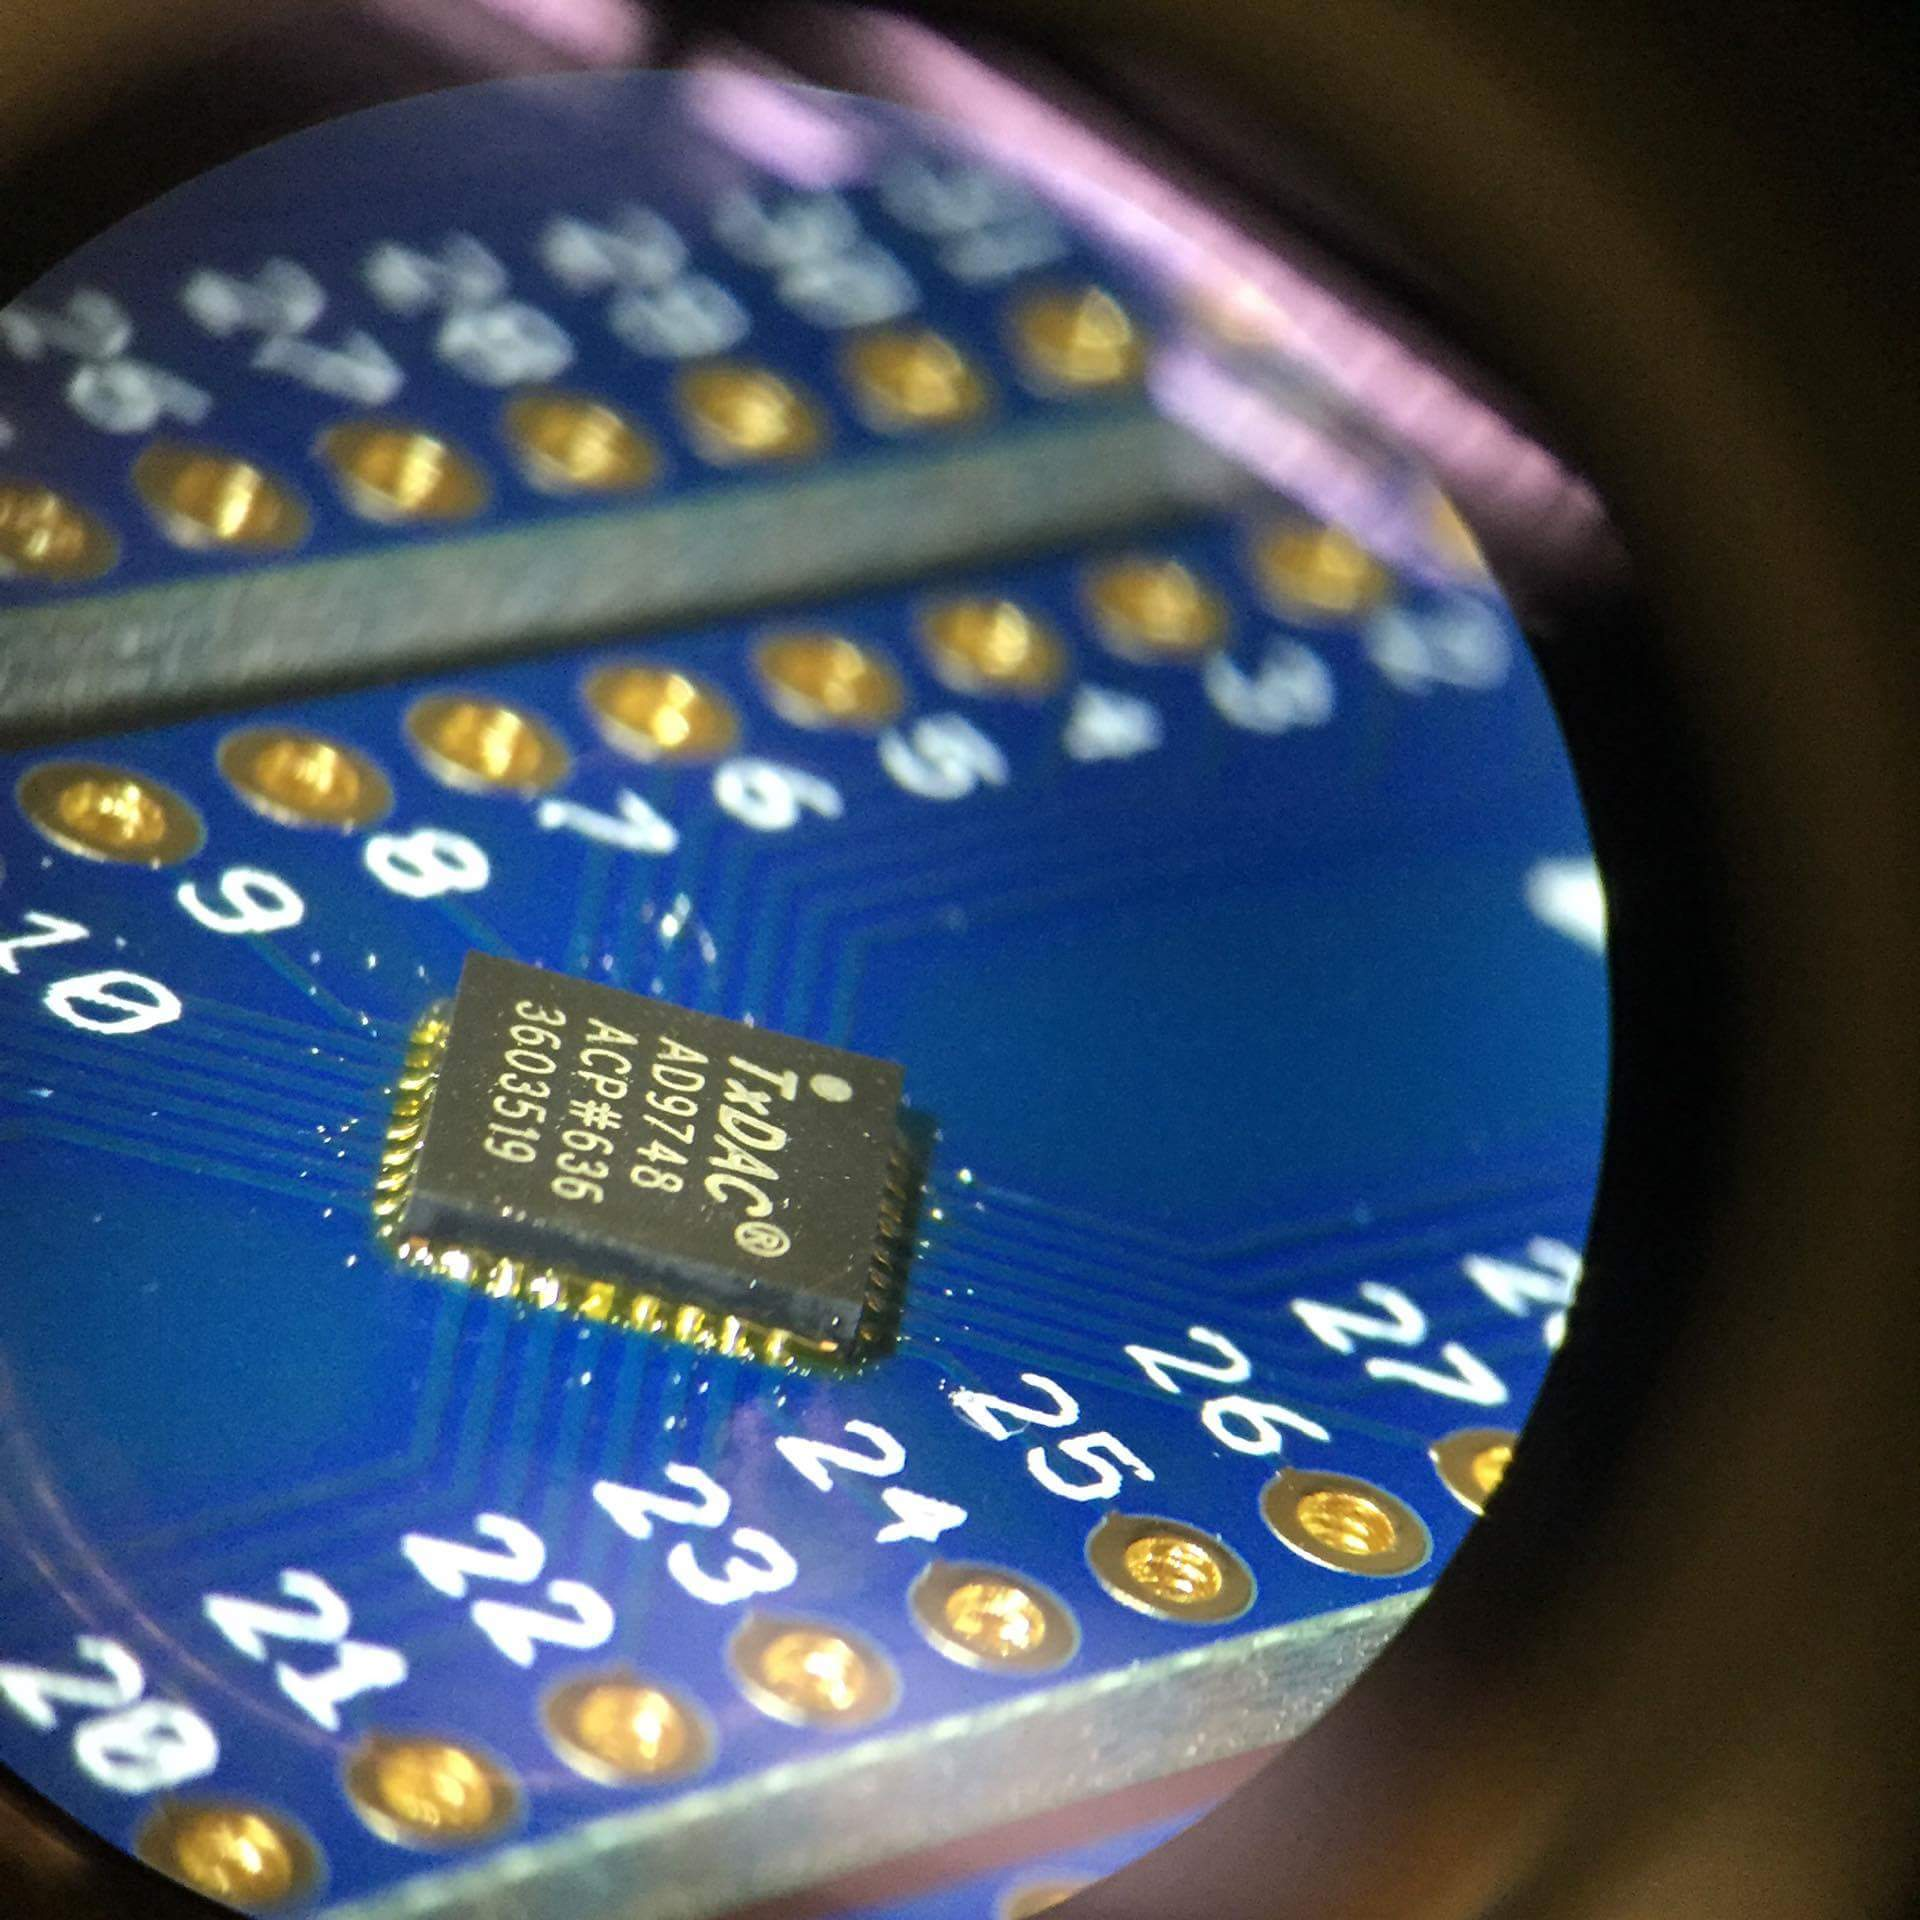
\includegraphics[scale=0.1]{surfaceMount.jpg}
    \caption{Surface Mounted DAC IC}
\end{figure}

As this DAC was going to be operated at 50 MSPS, the clock was put in
differential mode, and a shielded twisted pair was used as the connection
between the FPGA and the DAC board. This was to reduce any possible noise.
additionally the analog power was given a separate regulator that recieved
power from the external dual power supply. The clock and digital power was taken
from the FPGA.

The dual supply is also used to power the video amplifier. This takes the
differential current output of the DAC and converts it into the appropriate
range for composite video (-1V to 1V). The output of the amplifier is connected
to an RCA jack so that it can be easily connected to standard televisions.
Standard value resistors were used for the video amplifier while a potentiometer
was used to adjust the full scale range of the current output of the DAC.

In application we would not be using an external dual power supply but a switching
regulator. This keeps the package size down while only requiring a single power
supply. Additionally the switching power supply would provide some noise
immunity from harmonics created by the 50 MHz clock.

The circuit diagram for the prototype board is found in the appendix.

\begin{figure}[H]
    \centering
    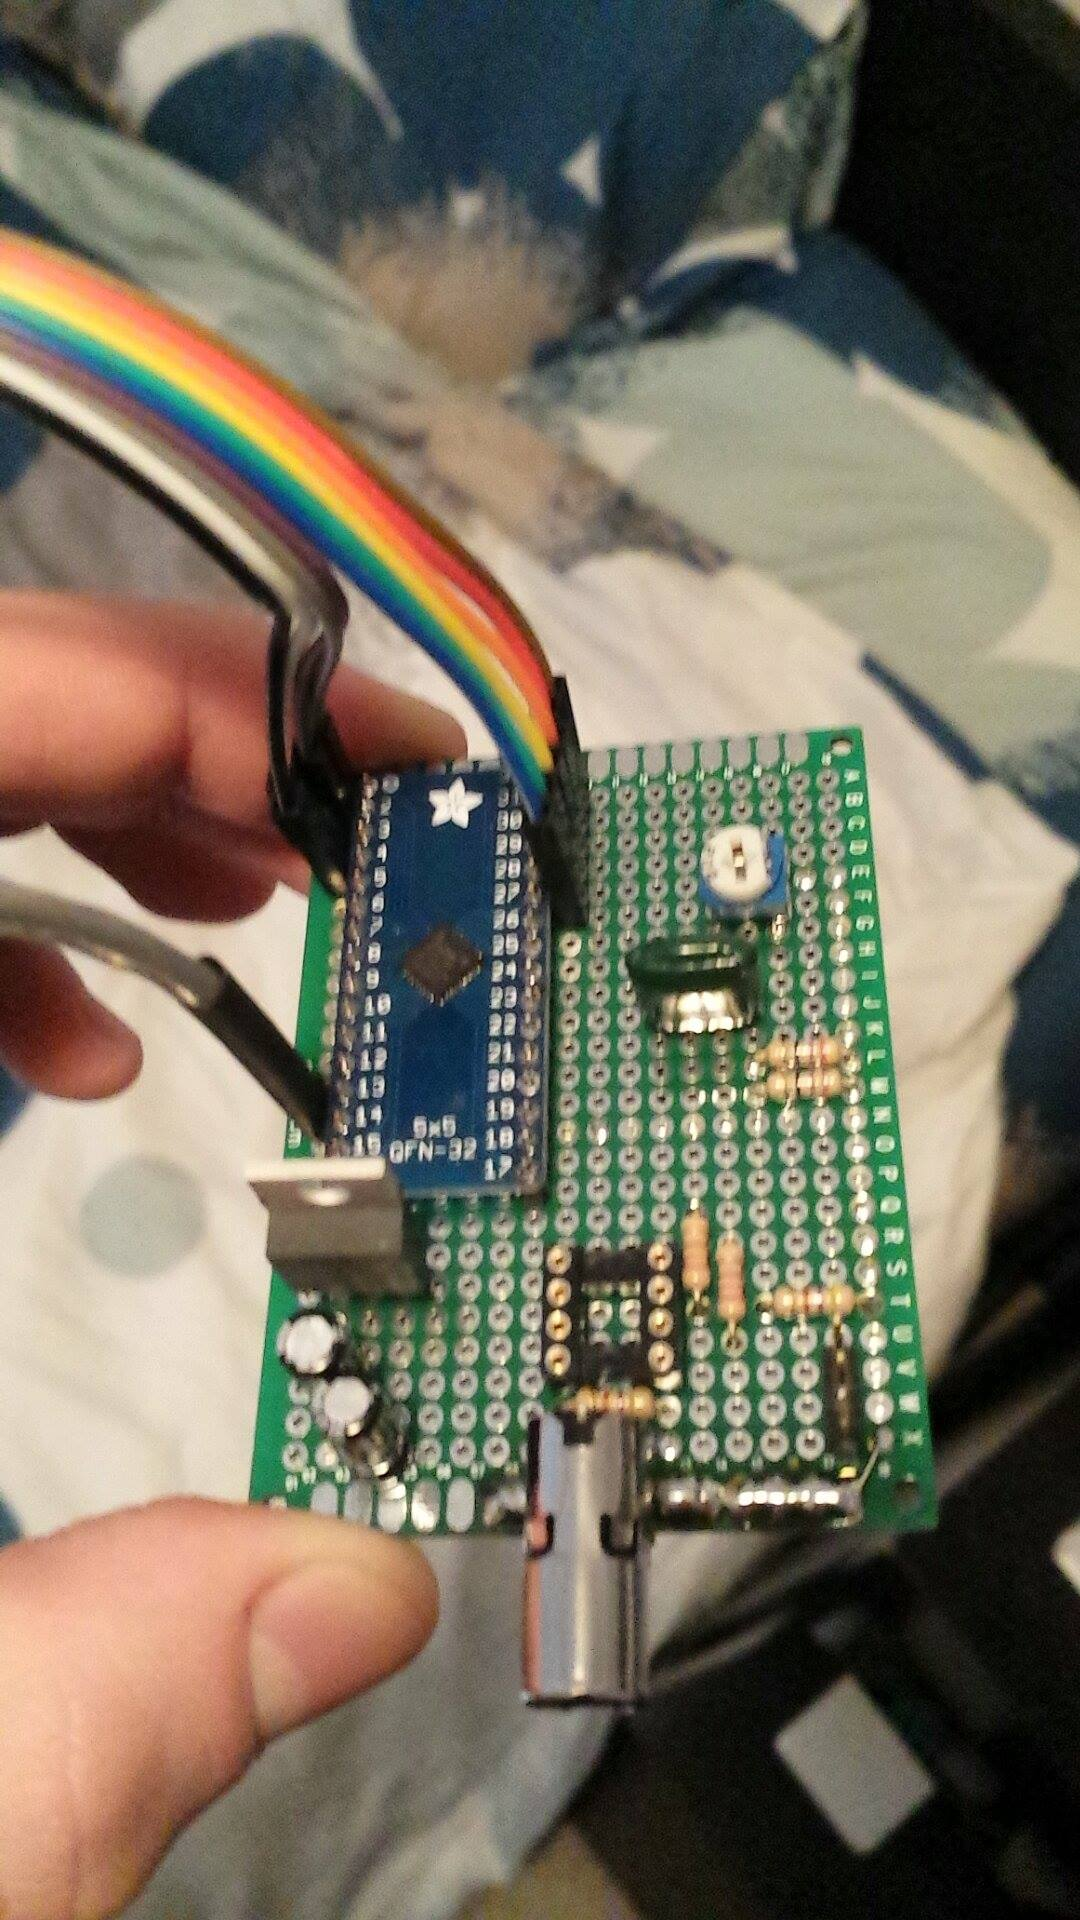
\includegraphics[scale=0.1]{protoBoard.jpg}
    \caption{}
\end{figure}

\subsection{Composite Driver}

\subsubsection{Timing Control}

\subsubsection{Line Buffer}

\subsubsection{Colour Modulation}

\subsection{SPI Module}

The SPI module was designed to take a 9-bit input and a clock input. 8 of the
9 bits was to indicate colour. The last bit was for internal communication. 
Internal communication included setting individual pixels, resetting the frame 
and any other special features the input device could use. Our SPI module was
designed this way so any device, slow or fast, could be used as an input.

Once the SPI module obtained an input, the module would stack two input pixels
and store the input on an array 320 elements long. Each element on the array 
would store 16-bits or two pixels. This make for easy conversion to the SDRAM.
The SDRAM stores 16 bits worth of data at a time.


\subsection{RAM Interface}

The RAM interface was not completed. Although to get this working we would 
needed to use NIOS 2 software to give us a file to be able to access the 
SDRAM. Once this Verilog file would be created we would have to modify it to
fit our needs and properly implement it in our system.


